\begin{figure}[htb]
\centering
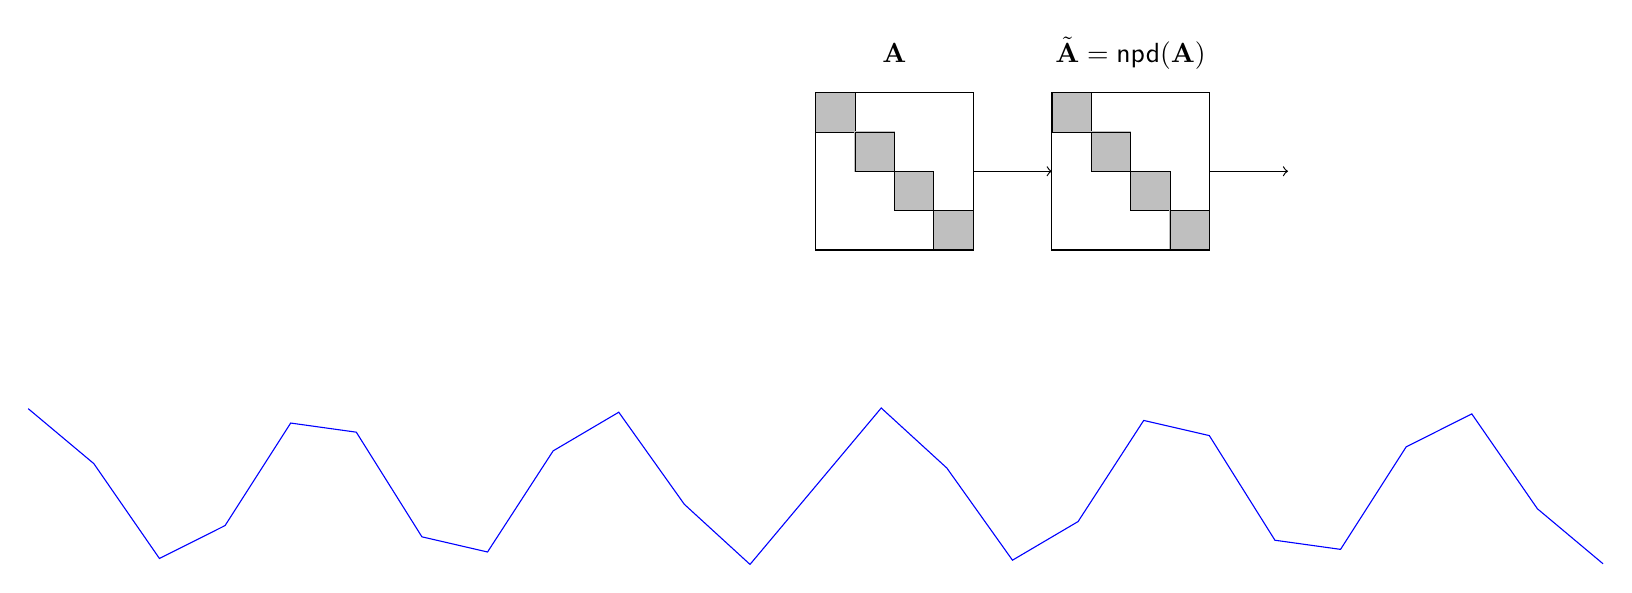
\begin{tikzpicture}
\def\cradius{1.5};
\def\cliqueradius{0.001};
%\draw[help lines,step=1] (0,0) grid (10,10);

\node at (1,2.5) {$\mathbf{A}$};
%\fill [white, draw] (0,0) rectangle (2,2);
\foreach \k in {0,0.5,...,1.5}{
\fill [gray!50,draw] (\k,-\k + 1.5) rectangle (\k+0.5,-\k + 2);
\draw [draw, line width=0.05ex] (\k,-\k + 1.5) rectangle (\k+0.5,-\k + 2);
}
\draw [black, draw] (0,0) rectangle (2,2);
\draw [->,line width=0.1ex] (2,1) -- (3,1);

\begin{scope}[shift={(3,0)}]
\node at (1,2.5) {$\tilde{\mathbf{A}}=\textsf{npd}(\mathbf{A})$};
%\fill [white, draw] (0,0) rectangle (2,2);
\foreach \k in {0,0.5,...,1.5}{
\fill [gray!50,draw] (\k,-\k + 1.5) rectangle (\k+0.5,-\k + 2);
\draw [draw, line width=0.05ex] (\k,-\k + 1.5) rectangle (\k+0.5,-\k + 2);
}
\draw [black, draw] (0,0) rectangle (2,2);
\draw [->,line width=0.1ex] (2,1) -- (3,1);
\end{scope}


\begin{scope}[shift={(0,-3)}]
\draw[scale=1,domain=-10:10,variable=\x,blue] plot({\x},{sin(\x*100)});
\end{scope}

\end{tikzpicture}
\caption{Workflow}
\end{figure}